\documentclass[a4paper]{article}
\usepackage[affil-it]{authblk}
\usepackage{amsthm,amsmath,amssymb}
\usepackage{geometry}
\usepackage{hyperref}
\usepackage{tikz}
\geometry{margin=1.5cm, vmargin={0pt,1cm}}
\setlength{\topmargin}{-1cm}
\setlength{\paperheight}{29.7cm}
\setlength{\textheight}{25.3cm}
\renewcommand{\qed}{\hfill \boxed{\mathbb{Q.E.D.}}}

\tikzset{elegant/.style={smooth,thick,solid,black}}
\tikzset{eaxis/.style={smooth,thick,solid,black}}
\begin{document}
% =================================================
\title{Numerical Analysis Homework 3}

\author{Chen Wanqi 3220102895
  \thanks{Electronic address: \texttt{3220102895@zju.edu.cn}}}
\affil{Information and Computer Science 2201, Zhejiang University }


\date{\today}

\maketitle

% =============================================== 
\section*{Problem I.}

\textbf{Solution.}

To satisfy the continuity and smoothness conditions at \( x = 1 \), the polynomial \( p(x) \) must meet the following constraints:
\[
p(0) = 0, \quad p(1) = 1, \quad p'(1) = -3, \quad p''(1) = 6.
\]
Using Hermite interpolation, we find that
\[
\boxed{p(x) = 7x^3 - 18x^2 + 12x}.
\]
To determine if \( s(x) \) is a natural cubic spline, we check the boundary condition for the second derivative at \( x = 0 \). For \( s(x) \) to be a natural cubic spline, \( s''(0) \) must equal zero. However, we compute
\[
s''(0) = -36 \neq 0,
\]
so \( s(x) \) is \boxed{not} a natural cubic spline.

% =============================================== 
\section*{Problem II.}

\subsection*{(a)}

\textbf{Proof.}

Since \( p_i = s|_{[x_i, x_{i+1}]} \in \mathbb{P}_2 \) for each interval \([x_i, x_{i+1}]\), there are \(3(n - 1)\) unknown coefficients for \(p_1, \ldots, p_{n-1}\). The conditions
\[
p_i(x_i) = f_i, \quad p_i(x_{i+1}) = f_{i+1} \quad \text{for } i = 1, \ldots, n - 1
\]
yield \(2(n - 1)\) equations. Additionally, the continuity of the first derivative at each interior point \(x_{i+1}\) provides
\[
p'_i(x_{i+1}) = p'_{i+1}(x_{i+1}) \quad \text{for } i = 1, \ldots, n - 2,
\]
giving \(n - 2\) more equations. In total, there are \(3(n - 1)\) unknowns and \(3(n - 1) - 1\) equations, so one additional condition is needed for a unique solution.

\qed

\subsection*{(b)}

\textbf{Solution.}

Let \( p_i(x) = a_i x^2 + b_i x + c_i \) on \([x_i, x_{i+1}]\). The conditions on \( p_i \) give:
\[
\begin{cases}
a_i x_i^2 + b_i x_i + c_i = f_i, \\
a_i x_{i+1}^2 + b_i x_{i+1} + c_i = f_{i+1}, \\
2 a_i x_i + b_i = m_i.
\end{cases}
\]
Solving these equations, we find:
\[
\begin{aligned}
a_i &= \frac{f_{i+1} - f_i}{(x_{i+1} - x_i)^2} - \frac{m_i}{x_{i+1} - x_i}, \\
b_i &= \frac{m_i (x_{i+1} + x_i)}{x_{i+1} - x_i} - \frac{2 x_i (f_{i+1} - f_i)}{(x_{i+1} - x_i)^2}, \\
c_i &= f_i + \frac{x_i^2 (f_{i+1} - f_i)}{(x_{i+1} - x_i)^2} - \frac{m_i x_i x_{i+1}}{x_{i+1} - x_i}.
\end{aligned}
\]

Finally we get, 
\[
\boxed{
p_i(x) = [\frac{f_{i+1} - f_i}{(x_{i+1} - x_i)^2} - \frac{m_i}{x_{i+1} - x_i}] x^2 + [\frac{m_i (x_{i+1} + x_i)}{x_{i+1} - x_i} - \frac{2 x_i (f_{i+1} - f_i)}{(x_{i+1} - x_i)^2}] x + [f_i + \frac{x_i^2 (f_{i+1} - f_i)}{(x_{i+1} - x_i)^2} - \frac{m_i x_i x_{i+1}}{x_{i+1} - x_i}]
}
\]

\subsection*{(c)}

\textbf{Solution.}

Starting with \( p_1 \) calculated using \( f_1 \), \( f_2 \), and \( m_1 \), we set \( m_2 = p'_1(x_2) \). 

With \( m_2 \), we compute \( p_2 \) using \( f_2 \), \( f_3 \), and set \( m_3 = p'_2(x_3) \). 

Repeating this process through \( p_{n-1} \) with \( f_{n-1} \), \( f_n \), and \( m_{n-1} \) completes the calculations.

% =============================================== 
\section*{Problem III.}

\textbf{Solution.}

Consider \( s_2(x) = \alpha x^3 + \beta x^2 + \gamma x + \theta \). The following conditions must be satisfied:
\[
s_2(0) = s_1(0) = 1 + c, \quad s'_2(0) = s'_1(0) = 3c, \quad s''_2(0) = s''_1(0) = 6c, \quad s_2(1) = s(1) = -1, \quad s''_2(1) = 0.
\]
These conditions lead to the system:
\[
\begin{cases}
\theta = 1 + c, \\
\gamma = 3c, \\
2\beta = 6c, \\
\alpha + \beta + \gamma + \theta = -1, \\
6\alpha + 2\beta = 0
\end{cases}.
\]
Solving this system yields \boxed{ c = -\frac{1}{3} }.

% =============================================== 
\section*{Problem IV.}

\textbf{Solution.}

\subsection*{(a)}
To construct the natural cubic spline \( s(x) \) that interpolates \( f(x) = \cos\left(\frac{\pi}{2}x\right) \) at the knots \(-1\), \(0\), and \(1\), we divide the interval \([-1,1]\) into two segments, \([-1,0]\) and \([0,1]\), and define \( s(x) \) piecewise over these intervals.

The natural cubic spline \( s(x) \) must satisfy the following conditions:

   \[
   s(-1) = f(-1) = 0, \quad s(0) = f(0) = 1, \quad s(1) = f(1) = 0.
   \]

   \[
   s'_1(0) = s'_2(0).
   \]

   \[
   s''_1(0) = s''_2(0).
   \]

   \[
   s''(-1) = 0, \quad s''(1) = 0.
   \]

Using these conditions, we find that the natural cubic spline interpolant \( s(x) \) is given by:
\[
\
s(x) = \begin{cases} 
-\frac{1}{2}x^3 - \frac{3}{2}x^2 + 1 & \text{for } x \in [-1,0], \\ 
\frac{1}{2}x^3 - \frac{3}{2}x^2 + 1 & \text{for } x \in [0,1].
\end{cases}
\]

\subsection*{(b)}
The bending energy of \( s \) is calculated as:
\[
\int_{-1}^1 [s''(x)]^2 \, dx = \int_{-1}^0 (-3x - 3)^2 \, dx + \int_{0}^1 (3x - 3)^2 \, dx = 6.
\]

The quadratic polynomial interpolating \( f \) at \(-1\), \(0\), and \(1\) is:
\[
p(x) = -x^2 + 1.
\]
Its bending energy is:
\[
\int_{-1}^1 [p''(x)]^2 \, dx = \int_{-1}^1 4 \, dx = 8 > 6.
\]

The bending energy of \( f \) is:
\[
\int_{-1}^1 [f''(x)]^2 \, dx = \int_{-1}^1 \left[-\frac{\pi^2}{4} \cos\left(\frac{\pi}{2} x\right)\right]^2 \approx \frac{\pi^4}{16} \approx 6.0881 > 6.
\]

Thus, the natural cubic spline \( s(x) \) has minimal bending energy among the functions considered.

% =============================================== 
\section*{Problem V.}

\textbf{Solution.}

\subsection*{(a)}
See that 
\[
B_i^1(x) = 
\begin{cases} 
    \frac{x - t_{i-1}}{t_i - t_{i-1}} & x \in (t_{i-1}, t_i], \\
    \frac{t_{i+1} - x}{t_{i+1} - t_i} &  x \in (t_i, t_{i+1}], \\
    0 & \text{other}.
\end{cases}
\]
\[
B_{i+1}^1(x) = 
\begin{cases} 
    \frac{x - t_i}{t_{i+1} - t_i} &  x \in (t_i, t_{i+1}], \\ 
    \frac{t_{i+2} - x}{t_{i+2} - t_{i+1}} &  x \in (t_{i+1}, t_{i+2}], \\ 
    0 & \text{other}.
\end{cases}
\]

By the recursive definition, we have
\[
B_i^2(x) = \frac{x - t_{i-1}}{t_{i+1} - t_{i-1}} B_i^1(x) + \frac{t_{i+2} - x}{t_{i+2} - t_i} B_{i+1}^1(x).
\]

For \(x \in (t_{i-1}, t_i]\),
\[
B_i^2(x) = \frac{x - t_{i-1}}{t_{i+1} - t_{i-1}} \cdot \frac{x - t_{i-1}}{t_i - t_{i-1}} + \frac{t_{i+2} - x}{t_{i+2} - t_i} \cdot 0 = \frac{(x - t_{i-1})^2}{(t_{i+1} - t_{i-1})(t_i - t_{i-1})}.
\]

For \(x \in (t_i, t_{i+1}]\),
\[
B_i^2(x) = \frac{(x - t_{i-1})(t_{i+1} - x)}{(t_{i+1} - t_{i-1})(t_{i+1} - t_i)} + \frac{(t_{i+2} - x)(x - t_i)}{(t_{i+2} - t_i)(t_{i+1} - t_i)}.
\]

For \(x \in (t_{i+1}, t_{i+2}]\),
\[
B_i^2(x) = \frac{x - t_{i-1}}{t_{i+1} - t_{i-1}} \cdot 0 + \frac{t_{i+2} - x}{t_{i+2} - t_i} \cdot \frac{t_{i+2} - x}{t_{i+2} - t_{i+1}} = \frac{(t_{i+2} - x)^2}{(t_{i+2} - t_i)(t_{i+2} - t_{i+1})}.
\]

Hence we derived
\[
B_i^2(x) = 
\begin{cases} 
    \frac{(x - t_{i-1})^2}{(t_{i+1} - t_{i-1})(t_i - t_{i-1})} &  x \in (t_{i-1}, t_i], \\ 
    \frac{(x - t_{i-1})(t_{i+1} - x)}{(t_{i+1} - t_{i-1})(t_{i+1} - t_i)} + \frac{(t_{i+2} - x)(x - t_i)}{(t_{i+2} - t_i)(t_{i+1} - t_i)} &  x \in (t_i, t_{i+1}], \\ 
    \frac{(t_{i+2} - x)^2}{(t_{i+2} - t_i)(t_{i+2} - t_{i+1})} &  x \in (t_{i+1}, t_{i+2}], \\ 
    0 & \text{other}.
\end{cases}
\]

\subsection*{(b)}
We have
\[
\frac{\text{d}}{\text{d}x}B_i^2(x) = 
\begin{cases} 
    p_1(x) = \frac{2(x-t_{i-1})}{(t_{i+1}-t_{i-1})(t_i-t_{i-1})} & x \in (t_{i-1}, t_i], \\ 
    p_2(x) = \frac{t_{i+1}+t_{i-1}-2x}{(t_{i+1}-t_{i-1})(t_{i+1}-t_i)} + \frac{t_{i+2}+t_i-2x}{(t_{i+2}-t_i)(t_{i+1}-t_i)} & x \in (t_i, t_{i+1}], \\ 
    p_3(x) = \frac{2(x-t_{i+2})}{(t_{i+2}-t_i)(t_{i+2}-t_{i+1})} & x \in (t_{i+1}, t_{i+2}], \\ 
    0 & \text{other}.
\end{cases}
\]

Next, evaluating the derivatives at the boundary points yields:
\begin{align*}
    p_1(t_i) & = \frac{2(t_i-t_{i-1})}{(t_{i+1}-t_{i-1})(t_i-t_{i-1})} = \frac{2}{t_{i+1}-t_{i-1}}, \\
    p_2(t_i) & = \frac{t_{i+1}+t_{i-1}-2t_i}{(t_{i+1}-t_{i-1})(t_{i+1}-t_i)} + \frac{t_{i+2}+t_i-2t_i}{(t_{i+2}-t_i)(t_{i+1}-t_i)} \\
              & = \frac{t_{i-1}-t_i}{(t_{i+1}-t_{i-1})(t_{i+1}-t_i)} + \frac{1}{t_{i+1}-t_{i-1}} + \frac{1}{t_{i+1}-t_i} \\
              & = \frac{2}{t_{i+1}-t_{i-1}} = p_1(t_i).
\end{align*}
This shows that \(\frac{\text{d}}{\text{d}x}B_i^2(x)\) is continuous at \(t_i\). 

Similarly, we find:
\begin{align*}
    p_3(t_{i+1}) & = \frac{2(t_{i+1}-t_{i+2})}{(t_{i+2}-t_i)(t_{i+2}-t_{i+1})} = -\frac{2}{t_{i+2}-t_i}, \\
    p_2(t_{i+1}) & = \frac{t_{i+1}+t_{i-1}-2t_{i+1}}{(t_{i+1}-t_{i-1})(t_{i+1}-t_i)} + \frac{t_{i+2}+t_i-2t_{i+1}}{(t_{i+2}-t_i)(t_{i+1}-t_i)} = -\frac{2}{t_{i+2}-t_i} = p_3(t_{i+1}).
\end{align*}
Thus, \(\frac{\text{d}}{\text{d}x}B_i^2(x)\) is also continuous at \(t_{i+1}\).


\subsection*{(c)}
It is established that \(\frac{\text{d}}{\text{d}x}B_i^2(x)\) maintains continuity and is a linear function across the intervals \((t_{i-1}, t_i]\), \((t_i, t_{i+1}]\), and \((t_{i+1}, t_{i+2}]\). We observe:

\[
\frac{\text{d}}{\text{d}x}B_i^2(t_{i-1}) = 0, \quad \text{and} \quad \frac{\text{d}}{\text{d}x}B_i^2(t_i) = \frac{2}{t_{i+1}-t_{i-1}} > 0.
\]

This implies that within the interval \((t_{i-1}, t_i]\):

\[
\frac{\text{d}}{\text{d}x}B_i^2(x) > 0.
\]

In addition, we find:

\[
\frac{\text{d}}{\text{d}x}B_i^2(t_{i+1}) = -\frac{2}{t_{i+2}-t_i} < 0.
\]

Therefore, by the behavior of linear functions, there exists a unique point \(x^* \in (t_i, t_{i+1})\) where \(\frac{\text{d}}{\text{d}x}B_i^2(x^*) = 0\). This leads to the equation:

\[
\frac{t_{i+1}+t_{i-1}-2x^*}{t_{i+1}-t_{i-1}} + \frac{t_{i+2}+t_i-2x^*}{t_{i+2}-t_i} = 0.
\]

Solving this equation gives us:

\[
x^* = \frac{t_{i+2}t_{i+1} - t_it_{i-1}}{(t_{i+2}+t_{i+1}) - (t_i+t_{i-1})}.
\]

\subsection*{(d)}

From part (c), we have established:

\[
\frac{\text{d}}{\text{d}x}B_i^2(x) > 0, \quad x \in (t_{i-1}, x^*)
\]
\[
\frac{\text{d}}{\text{d}x}B_i^2(x) < 0, \quad x \in (x^*, t_{i+2}).
\]

Additionally, we note that \(B_i^2(t_{i-1}) = B_i^2(t_{i+2}) = 0\). A simple computation confirms that \(B(x^*) < 1\). Therefore, it follows that \(B_i^2(x) \in [0, 1)\).

\subsection*{(e)}

It is evident that the graphs of \(B_i^2(x)\) for different values of \(i\) can be generated through translations. Thus, we will illustrate the case for \(i = 0\).

\begin{center}
    \begin{tikzpicture}
        \draw[eaxis] (-1.5,0) -- (2.5,0) node[below] {$x$};
        \draw[eaxis] (0,-0.2) -- (0,1.2) node[above] {$B_i^2(x)$};
        \draw[elegant,domain=-1.5:-1] plot(\x,0);
        \draw[elegant,domain=-1:0] plot(\x,{(\x+1)^2/2});
        \draw[elegant,domain=0:1] plot(\x,{(\x+1)*(1-\x)/2+(2-\x)*\x/2});
        \draw[elegant,domain=1:2] plot(\x,{(2-\x)^2/2});
        \draw[elegant,domain=2:2.5] plot(\x,0);
    \end{tikzpicture}
\end{center}

\qed

\section*{Problem VI.}

\textbf{Proof.}


For \( x \in (t_{i-1}, t_i] \), applying Lagrange's interpolation formula yields:

\begin{align*}
    [t_{i-1}, t_i, t_{i+1}, t_{i+2}](t - x)_+^2 = & \frac{(t_i - x)^2}{(t_i - t_{i-1})(t_i - t_{i+1})(t_i - t_{i+2})} + \frac{(t_{i+1} - x)^2}{(t_{i+1} - t_{i-1})(t_{i+1} - t_i)(t_{i+1} - t_{i+2})} \\
    & + \frac{(t_{i+2} - x)^2}{(t_{i+2} - t_{i-1})(t_{i+2} - t_i)(t_{i+2} - t_{i+1})} \\
    = & \frac{(x - t_{i-1})^2}{(t_{i+2} - t_{i-1})(t_{i+1} - t_{i-1})(t_i - t_{i-1})} = \frac{B_i^2(x)}{t_{i+2} - t_{i-1}}.
\end{align*}

For \( x \in (t_i, t_{i+1}] \), we similarly have:

\begin{align*}
    [t_{i-1}, t_i, t_{i+1}, t_{i+2}](t - x)_+^2 = & \frac{(t_{i+1} - x)^2}{(t_{i+1} - t_{i-1})(t_{i+1} - t_i)(t_{i+1} - t_{i+2})} + \frac{(t_{i+2} - x)^2}{(t_{i+2} - t_{i-1})(t_{i+2} - t_i)(t_{i+2} - t_{i+1})} \\
    = & \frac{B_i^2(x)}{t_{i+2} - t_{i-1}}.
\end{align*}

For \( x \in (t_{i+1}, t_{i+2}] \), we find:

\begin{align*}
    [t_{i-1}, t_i, t_{i+1}, t_{i+2}](t - x)_+^2 = & \frac{(t_{i+2} - x)^2}{(t_{i+2} - t_{i-1})(t_{i+2} - t_i)(t_{i+2} - t_{i+1})} \\
    = & \frac{B_i^2(x)}{t_{i+2} - t_{i-1}}.
\end{align*}

Thus, we have confirmed that

\[
(t_{i+2} - t_{i-1})[t_{i-1}, t_i, t_{i+1}, t_{i+2}](t - x)_+^2 = B_i^2(x)
\]

holds true within the support of \( B_i^2(x) \). Moreover, this equation is evidently valid even when \( B_i^2(x) \) is equal to zero.

\qed

\section*{Problem VII.}

\textbf{Solution.}

According to the theorem on B-spline derivatives, we have:

\[
\frac{\text{d}}{\text{d}x} B_i^{n+1}(x) = \frac{(n+1) B_i^n(x)}{t_{i+n} - t_{i-1}} - \frac{(n+1) B_{i+1}^n(x)}{t_{i+n+1} - t_i}, \quad n \geq 1
\]

Integrating both sides results in:

\[
\int_{t_{i-1}}^{t_{i+n+1}} \frac{\text{d}}{\text{d}x} B_i^{n+1}(x) \, \text{d}x = \int_{t_{i-1}}^{t_{i+n+1}} \left( \frac{(n+1) B_i^n(x)}{t_{i+n} - t_{i-1}} - \frac{(n+1) B_{i+1}^n(x)}{t_{i+n+1} - t_i} \right) \text{d}x
\]

For the left-hand side, we have:

\[
\text{LHS} = B_i^{n+1}(t_{i+n+1}) - B_i^{n+1}(t_{i-1}) = 0.
\]

For the right-hand side, this yields:

\[
\text{RHS} = (n+1) \left( \int_{t_{i-1}}^{t_{i+n}} \frac{B_i^n(x)}{t_{i+n} - t_{i-1}} \, \text{d}x - \int_{t_i}^{t_{i+n+1}} \frac{B_{i+1}^n(x)}{t_{i+n+1} - t_i} \, \text{d}x \right).
\]

Therefore, we obtain:

\[
\int_{t_{i-1}}^{t_{i+n}} \frac{B_i^n(x)}{t_{i+n} - t_{i-1}} \, \text{d}x = \int_{t_i}^{t_{i+n+1}} \frac{B_{i+1}^n(x)}{t_{i+n+1} - t_i} \, \text{d}x.
\]

Consequently, the scaled integral of \( B_i^n(x) \) across its support is independent of the index \( i \).


\section*{Problem VIII.}

\textbf{Solution.}

\subsection*{(a)}
Firstly, we have:

\[
\tau_2(x_i, x_{i+1}, x_{i+2}) = x_i^2 + x_{i+1}^2 + x_{i+2}^2 + x_ix_{i+1} + x_ix_{i+2} + x_{i+1}x_{i+2}.
\]

Next, we can create a divided difference table as follows:

\begin{table}[h]
    \centering
    \begin{tabular}{l|lll}
        $x_i$     & $x_i^4$     &                                          &                                                                                                 \\
        $x_{i+1}$ & $x_{i+1}^4$ & $(x_{i+1}^2 + x_i^2)(x_{i+1} + x_i)$     &                                                                                                 \\
        $x_{i+2}$ & $x_{i+2}^4$ & $(x_{i+2}^2 + x_{i+1}^2)(x_{i+2} + x_{i+1})$ & $\frac{(x_{i+2}^2 + x_{i+1}^2)(x_{i+2} + x_{i+1}) - (x_{i+1}^2 + x_i^2)(x_{i+1} + x_i)}{x_{i+2} - x_i}$
    \end{tabular}
\end{table}

From the above, we derive:

\begin{align*}
    & \frac{(x_{i+2}^2 + x_{i+1}^2)(x_{i+2} + x_{i+1}) - (x_{i+1}^2 + x_i^2)(x_{i+1} + x_i)}{x_{i+2} - x_i} \\
    = & \frac{(x_{i+2}^3 - x_i^3) + x_{i+1}(x_{i+2}^2 - x_i^2) + x_{i+1}^2(x_{i+2} - x_i)}{x_{i+2} - x_i} \\
    = & (x_{i+2}^2 + x_{i+2} x_i + x_i^2) + x_{i+1}(x_{i+2} + x_i) + x_{i+1}^2 \\
    = & \tau_2(x_i, x_{i+1}, x_{i+2}).
\end{align*}

\subsection*{(b)}
According to the properties of complete symmetric polynomials, we can express:

\begin{align*}
    & (x_{i+n+1} - x_i) \sigma_{m-n-1}(x_i, \ldots, x_{i+n+1}) \\
    = & \sigma_{m-n}(x_i, \ldots, x_{i+n+1}) - \sigma_{m-n}(x_i, \ldots, x_{i+n}) - x_i \sigma_{m-n-1}(x_i, \ldots, x_{i+n+1}) \\
    = & \sigma_{m-n}(x_{i+1}, \ldots, x_{i+n+1}) + x_i \sigma_{m-n-1}(x_i, \ldots, x_{i+n+1}) - \sigma_{m-n}(x_i, \ldots, x_{i+n}) - x_i \sigma_{m-n-1}(x_i, \ldots, x_{i+n+1}) \\
    = & \sigma_{m-n}(x_{i+1}, \ldots, x_{i+n+1}) - \sigma_{m-n}(x_i, \ldots, x_{i+n}).
\end{align*}

Next, we will demonstrate the theorem using mathematical induction. When \( n = 0 \), it is clear that:

\[
\sigma_m(x_i) = [x_i] x^m = x_i^m.
\]

Assuming the theorem holds for some \( 0 \leq n < m \), we now consider the case for \( n + 1 \):

\begin{align*}
    \sigma_{m-n-1}(x_i, \ldots, x_{i+n+1}) & = \frac{\sigma_{m-n}(x_{i+1}, \ldots, x_{i+n+1}) - \sigma_{m-n}(x_i, \ldots, x_{i+n})}{x_{i+n+1} - x_i} \\
    & = \frac{[x_{i+1}, \ldots, x_{i+n+1}] x^m - [x_i, \ldots, x_{i+n}]}{x_{i+n+1} - x_i} \\
    & = [x_i, \ldots, x_{i+n+1}] x^m.
\end{align*}

This completes the proof of the theorem via induction.

% =======================
\section*{References}
\begin{itemize}
   \item handoutsNumPDEs
   \item ChatGPT, *AI Language Model*, OpenAI Platform, 2024.
\end{itemize}

\end{document}